%% ============================================================
%% 分片 05：原文第 3 节「Topological Field Theory From ${\EUN}=4$ Super Yang-Mills Theory」（原文 glshort.tex 起于第 1216 行）
%% 由 tools/harvmac2tex.py 从 arXiv 源码（hep-th/0604151v3）自动生成。
%% 只译英文散文；公式、编号、\label、\cite 一律不改。
%% ============================================================

\subsection{扭化 ${\EUN}=4$ 超对称杨--米尔斯理论}

\label{sec:twisting}

\par\medskip{\it 扭化的一般想法}


${\EUN}=2$ 超对称杨--米尔斯理论可以扭化，从而给出 Donaldson 理论的量子场论实现 \cite{ref25}。类似地 \cite{ref45}，${\EUN}=4$ 超对称杨--米尔斯理论可以用三种方式扭化，得到拓扑场论。其中两种扭化理论——包括 \cite{ref45} 中详细研究过的那一种——与 Donaldson 理论密切类似，因为它们给出瞬子不变量，而这些不变量像四维流形的 Donaldson 不变量一样，可以用 Seiberg-Witten 不变量表示。第三种扭化曾在 \cite{ref52} 中提及，并在 \cite{ref53,ref54,ref55,ref56,ref57} 中得到研究，但此前一直没有应用。结果表明它正是与几何 Langlands 纲领相关的扭化，我们将称之为 GL 扭化。

\begin{yizhu}[易错点]
按：这里说的三种扭化，不要与 ${\EUN}=2$ 理论的 Donaldson--Witten 扭化混为一谈。对 ${\EUN}=4$ 而言，三种扭化对应同态 $\varkappa:Spin(4)\to Spin(6)$ 的三种不等价取法（相差 Weyl 群的作用）：其中两种给出与 Donaldson 理论类似的瞬子不变量，只有第三种——本文的 GL 扭化——与几何 Langlands 纲领有关。一个实用的判据是 $S^+$ 中保留几个 $Spin'(4)$-不变旋量：前两种各保留一个，GL 扭化保留的则是两个独立不变旋量张成的整个二维复空间（正是这一点使后文出现以 $\Bbb{CP}^1$ 为参数的扭化族）。
\end{yizhu}

为了给扭化的概念一个不可避免会非常简短的说明，我们首先取 $M=\Bbb{R}^4$。它的旋转对称群当然是 $Spin(4)$，而 ${\EUN}=4$ 理论具有更大的对称性 $Spin(4)\times Spin(6)$。「扭化」意味着把 $Spin(4)$ 换成 $Spin(4)\times Spin(6)$ 中另一个同构于 $Spin(4)$ 的子群 $Spin'(4)$：它在 $\Bbb{R}^4$ 上的作用与 $Spin(4)$ 相同，但在 ${\EUN}=4$ 规范理论上的作用不同。为做到这一点，我们取一个同态 $\varkappa:Spin(4)\to Spin(6)$，并令 $Spin'(4)=(1\times \varkappa)(Spin(4))\subset Spin(4)\times Spin(6)$。

\begin{yizhu}[物理图像]
按：扭化的物理图像可以概括为一句话：同一个量子场论，换一套「自旋」的定义。理论的场按 $Spin(4)\times Spin(6)$ 的表示变换；把 $Spin(4)$ 换成对角子群 $Spin'(4)=(1\times\varkappa)(Spin(4))$ 之后，原本按 $({\bf 2},\bone)$ 变换的超对称生成元在 $Spin'(4)$ 下变成标量（不变），于是它可以在任意弯曲流形上定义，相应的超荷 $Q$ 就是拓扑对称。Witten 2008 综述（《Mirror Symmetry, Hitchin's Equations, And Langlands Duality》）第 2 节说明的正是同一件事：${\EUN}=4$ 超对称规范理论经扭化后，其类 Higgs 标量场变成 Hitchin 方程中的 Higgs 场。本文特别之处在于：扭化之后 $S^+$ 中留下两个独立的不变旋量，因此可选的 $Q$ 构成一整族。
\end{yizhu}

我们还希望选取 $\varkappa$，使得 $Spin'(4)$ 在 ${\EUS}^+$ 上的作用有一个非零的不变向量。由于超对称生成元 $\epsilon$ 取值于 ${\EUS}^+$，在 ${\EUS}^+$ 中选取一个不变向量，就给出一个 $Spin'(4)$-不变的超对称，我们称它为 $Q$。由式~\eqref{eq:ugo}，它将自动满足 $Q^2=0$。（式~\eqref{eq:ugo} 的右边没有 $Spin'(4)$ 不变算子；而 $Q^2=\half\{Q,Q\}$ 是 $Spin'(4)$-不变的，故它必须为零。）一旦选定了 $Q$，我们就改变理论的物理解释：只关心 $Q$-不变的路径积分、算子与态，并把任何形如 $[Q,{\EUO}\}$ 的量（${\EUO}$ 为任意算子）视为平凡的。因此从此以后，有趣的算子或态都落在 $Q$ 的适当上同调群中。

\begin{yizhu}[含糊点拨]
按：$Q^2=0$ 的论证值得慢慢看。超对称代数中 $\{Q,Q\}$ 正比于平移生成元 $P_\mu$（式~\eqref{eq:ugo} 的右边正是 $\Gamma^\mu P_\mu$ 结构），所以裸的超荷平方并不为零。要点在于：$Spin'(4)$-不变意味着 $Q^2=\half\{Q,Q\}$ 也是 $Spin'(4)$-不变的；而扭化之后，$\Gamma^\mu P_\mu$ 这类算子不再含有 $Spin'(4)$ 的不变分量，于是这个不变算子只能是零。换句话说，$Q$ 成为标量超荷这件事与 $Q^2=0$ 是同一枚硬币的两面。后文 §6.4 讨论拓扑超荷的三种叫法（标量/拓扑/BRST）时会再回到这一点。
\end{yizhu}

结果表明，这样得到的理论松散地说是拓扑场论。（它们可能依赖于 $M$ 的光滑结构，因为光滑结构在扭化之前或之后进入了量子场论的定义。）其证明方式是：把理论在平坦 $\Bbb{R}^4$ 上的定义延拓到任意四维流形，使得 $Q$ 对称性得以保留，而度规的选取只差 $Q$-恰当项。对于 ${\EUN}=4$ 超对称杨--米尔斯理论的 GL 扭化，这一进路的一种做法可见 \cite{ref56} 第 7 节。在本文中我们走另一条路：一旦算出了拓扑方程与消灭定理，我们就会在第~\ref{sec:toplag}~节直接看出，弯曲四维流形上的哪个作用量具有正确的性质。

\par\medskip{\it 扭化的描述}

现在我们来描述 GL 扭化。同态 $\varkappa:Spin(4)\to Spin(6)$ 的选取使得 $Spin(6)=SU(4)_{{\cal R}}$ 的 ${\bf 4}$ 按 $Spin(4)=SU(2)\times SU(2)$ 的 $({\bf 2},\bone)\oplus(\bone,{\bf 2})$ 变换，我们把后者记作 $SU(2)_\ell\times SU(2)_\rr$。\footnote{$SU(2)_\ell$ 与 $SU(2)_\rr$ 中的「$\ell$」与「$r$」通常读作「左」与「右」，指物理无质量粒子的自旋。}（$Spin(6)$ 的 $\bar{\bf 4}$ 是 ${\bf 4}$ 的复共轭，它在 $Spin(4)$ 下按同样的方式变换，因为 $Spin(4)$ 的 $({\bf 2},\bone)$ 与 $(\bone,{\bf 2})$ 是伪实的。）

这一 $\varkappa$ 的选取相当于按如下方式把 $SU(2)_\ell\times SU(2)_\rr$ 嵌入 $Spin(6)=SU(4)_{{\cal R}}$：
% 式 (3.2)
\setcounter{equation}{1}
\begin{equation}\label{eq:norml}
\left(\begin{matrix}SU(2)_\ell &  0 \\
                                                  0    &
                                                  SU(2)_\rr\\\end{matrix}\right).
\end{equation}

这一嵌入显然与一个额外的 $U(1)$ 群交换，\footnote{这个联合群的全局结构其实不是乘积 $SU(2)_\ell\times SU(2)_\rr\times U(1)$，而是商 $(SU(2)_\ell\times SU(2)_\rr\times U(1))/\Bbb{Z}_2$。}我们可以把它的生成元 ${\cal K}$ 取为如下形式 % 式 (3.3)
\setcounter{equation}{2}
\begin{equation}\label{eq:orml}
{\cal K}=i\left(\begin{matrix}1&  0 \\
                                                  0    &
                                                  -1\\\end{matrix}\right)
\end{equation}

其中分 $2\times 2$ 块。于是我们的嵌入使得 $Spin(6)$ 的 ${\bf 4}$ 在 $SU(2)_\ell\times SU(2)_\rr\times U(1)$ 下按 $({\bf 2},\bone)^{1}\oplus(\bone,{\bf 2})^{-1}$ 变换；这里上标指数是 $-i{\cal K}$ 的本征值，我们称它为 ${\EUK}$。$\bar{\bf 4}$ 按上式的复共轭变换，即 $({\bf 2},\bone)^{-1}\oplus(\bone,{\bf 2})^{1}$。

\begin{yizhu}[易错点]
按：$({\bf 2},\bone)^{1}\oplus(\bone,{\bf 2})^{-1}$ 里的上标 $1,-1$ 是 $-i{\cal K}$ 的本征值 ${\EUK}$，而不是 ${\cal K}$ 本身的本征值——式~\eqref{eq:orml} 中 ${\cal K}$ 的定义带一个因子 $i$，所以 ${\cal K}$ 的本征值是 $i$ 与 $-i$，$-i{\cal K}$ 的本征值才是 $\pm 1$。这个约定贯穿全文：$\phi_\mu$ 的 ${\EUK}=0$，$\sigma,\bar\sigma$ 的 ${\EUK}=\pm 2$，扭化超荷的 ${\EUK}=1$，全部按此记账。另外 ${\bf 4}$ 与 $\bar{\bf 4}$ 的指数互为相反数：${\bf 4}$ 是 $({\bf 2},\bone)^{1}\oplus(\bone,{\bf 2})^{-1}$，$\bar{\bf 4}$ 是 $({\bf 2},\bone)^{-1}\oplus(\bone,{\bf 2})^{1}$，切勿混用。
\end{yizhu}

这个扭化也可以方便地用 $SO$ 群而不是 $Spin$ 群来描述。为此我们用到：$SO(6)$ 的基本六维矢量表示 ${\bf 6_v}$，用 $Spin(6)=SU(4)_{{\cal R}}$ 的语言来说，就是 $\wedge^2 {\bf 4}$，即 ${\bf 4}\otimes{\bf 4}$ 的反对称部分。于是 ${\bf 6_v}=\wedge^2(({\bf 2},\bone)^{1}\oplus(\bone,{\bf 2})^{-1})=(\btwo,\btwo)^0\oplus(\bone,\bone)^2\oplus(\bone,\bone)^{-2}$。这里 $(\btwo,\btwo)$ 就是 $SO(4)$ 的矢量表示 ${\bf 4_v}$。因此 ${\bf 6_v}$ 是一个 ${\EUK}=0$ 的 $SO(4)$ 矢量 ${\bf 4_v}$ 与两个 ${\EUK}=\pm 2$ 的 $SO(4)$ 标量之和。这对应于 $SO(4)\times U(1)=SO(4)\times SO(2)$ 到 $SO(6)$ 的显然同态：\footnote{$(SU(2)\times SU(2)\times U(1))/\Bbb{Z}_2\subset SU(4)$ 中的 $U(1)$ 是 $SO(4)\times U(1)\subset SO(6)$ 中 $U(1)$ 的双覆盖。} % 式 (3.4)
\setcounter{equation}{3}
\begin{equation}\label{eq:tomo}
\left(\begin{matrix}SO(4) &
0 \\ 0 & SO(2)\\\end{matrix}\right).
\end{equation}

${\EUN}=4$ 超对称杨--米尔斯理论的六个自旋为零的场 $\phi_i$（$i=0,\dots,5$）按 $SO(6)$ 的 ${\bf 6_v}$ 变换，因此上述分析适用于它们。我们可以选取坐标，使得前四个场 $\phi_0,\dots,\phi_3$ 构成 $SO(4)$ 的 ${\bf 4_v}$，而 $\phi_4$ 与 $\phi_5$ 是 $SO(4)$ 标量，它们在 $SO(2)$ 下转动。此外，我们可以对标量场作如下标号：使得线性组合 $\sigma=(\phi_4-i\phi_5)/\sqrt 2$ 与 $\bar\sigma=(\phi_4+i\phi_5)/\sqrt 2$ 分别具有 ${\EUK}=2$ 与 ${\EUK}=-2$。于是场 $\phi_0,\dots,\phi_3$ 可以在几何上解释为一个伴随丛取值的 1-形式的各个分量，而 $\sigma$ 是取值于李代数复化的标量场（零形式）。因此理论的玻色场是：一个规范场（局部上即伴随丛取值的 1-形式 $A=A_\mu \,dx^\mu$），以及第二个伴随丛取值的 1-形式 $\phi=\phi_\mu\,dx^\mu$，还有复标量 $\sigma$ 与 $\bar\sigma$。

\par\medskip{\it 超对称的变换}

我们同样可以分析超对称在 $Spin'(4)$ 下如何变换。$Spin(6)$ 的 $\bar{\bf 4}$ 按 $Spin'(4)\times U(1)$ 的 $({\bf 2},\bone)^{-1}\oplus(\bone,{\bf 2})^{1}$ 变换，而 ${\bf 4}$ 按 $({\bf 2},\bone)^{1}\oplus(\bone,{\bf 2})^{-1}$ 变换。于是利用式~\eqref{eq:jugo}，按 $Spin(4)$ 的 $({\bf 2},\bone)$ 变换的那些超对称，在 $Spin'(4)\times U(1)$ 下按如下方式变换： % 式 (3.5)
\setcounter{equation}{4}
\begin{equation}\label{eq:lollypop}
(\btwo,\bone)^0\otimes
((\btwo,\bone)^{-1}\oplus (\bone,\btwo)^{1}) =
(\bone,\bone)^{-1}\oplus ({\bf 3},\bone)^{-1}
\oplus(\btwo,\btwo)^{1}.
\end{equation}
而按 $Spin(4)$ 的 $(\bone,{\bf 2})$ 变换的那些超对称，在 $Spin'(4)\times U(1)$ 下按如下方式变换： % 式 (3.6)
\setcounter{equation}{5}
\begin{equation}\label{eq:tollypop}
(\bone,\btwo)^0\otimes
((\btwo,\bone)^{1}\oplus (\bone,\btwo)^{-1}) = (\bone,\bone)^{-1}
\oplus (\bone,{\bf 3})^{-1} \oplus(\btwo,\btwo)^{1}.
\end{equation}

接下来我们可以找出 $Spin'(4)$ 不变的那些超对称。由式~\eqref{eq:lollypop} 与式~\eqref{eq:tollypop}，存在一个在四维意义下为左手的（即在原 $Spin(4)$ 下按 $({\bf 2},\bone)$ 变换的）不变超对称生成元 $\epsilon_\ell$，以及一个这样的右手生成元 $\epsilon_\rr$（按 $(\bone,{\bf 2})$ 变换）。在我们的约定下，二者由下式区分：
% 式 (3.7)
\setcounter{equation}{6}
\begin{equation}\label{eq:onog}
\begin{aligned}\hat\Gamma_E\epsilon_\ell& = -\epsilon_\ell\\
\hat\Gamma_E\epsilon_\rr& = \epsilon_\rr.\\\end{aligned}
\end{equation}
$\epsilon_\ell$ 的选取决定了 $\epsilon_\rr$ 的一个自然选取，即 % 式 (3.8)
\setcounter{equation}{7}
\begin{equation}\label{eq:huy}
\epsilon_\rr=N\epsilon_\ell,
\end{equation}
其中 $N={1\over 4}\sum_{\mu=0}^3\Gamma_{\mu+4}\Gamma_{\mu}$。这里的想法是：$N$ 与 $Spin'(4)$ 交换，但与 $\hat\Gamma_E$ 反交换，因此定义~\eqref{eq:huy} 是合理的。我们已对 $N$ 作了归一化，使得当 $\epsilon$ 为 $Spin'(4)$-不变时 $N^2\epsilon=-\epsilon$。因此我们同样有
% 式 (3.9)
\setcounter{equation}{8}
\begin{equation}\label{eq:uy}
\epsilon_\ell=-N\epsilon_\rr.
\end{equation}
利用 $Spin'(4)$ 对称性可以证明，当 $\mu=0,\dots,3$ 时，我们有 % 式 (3.10)
\setcounter{equation}{9}
\begin{equation}\label{eq:uzu}
\Gamma_{\mu+4}\epsilon_\ell =
-\Gamma_\mu\epsilon_r,~\Gamma_{\mu+4}\epsilon_r=\Gamma_\mu\epsilon_\ell.
\end{equation}

\begin{figure}[htbp]
\centering
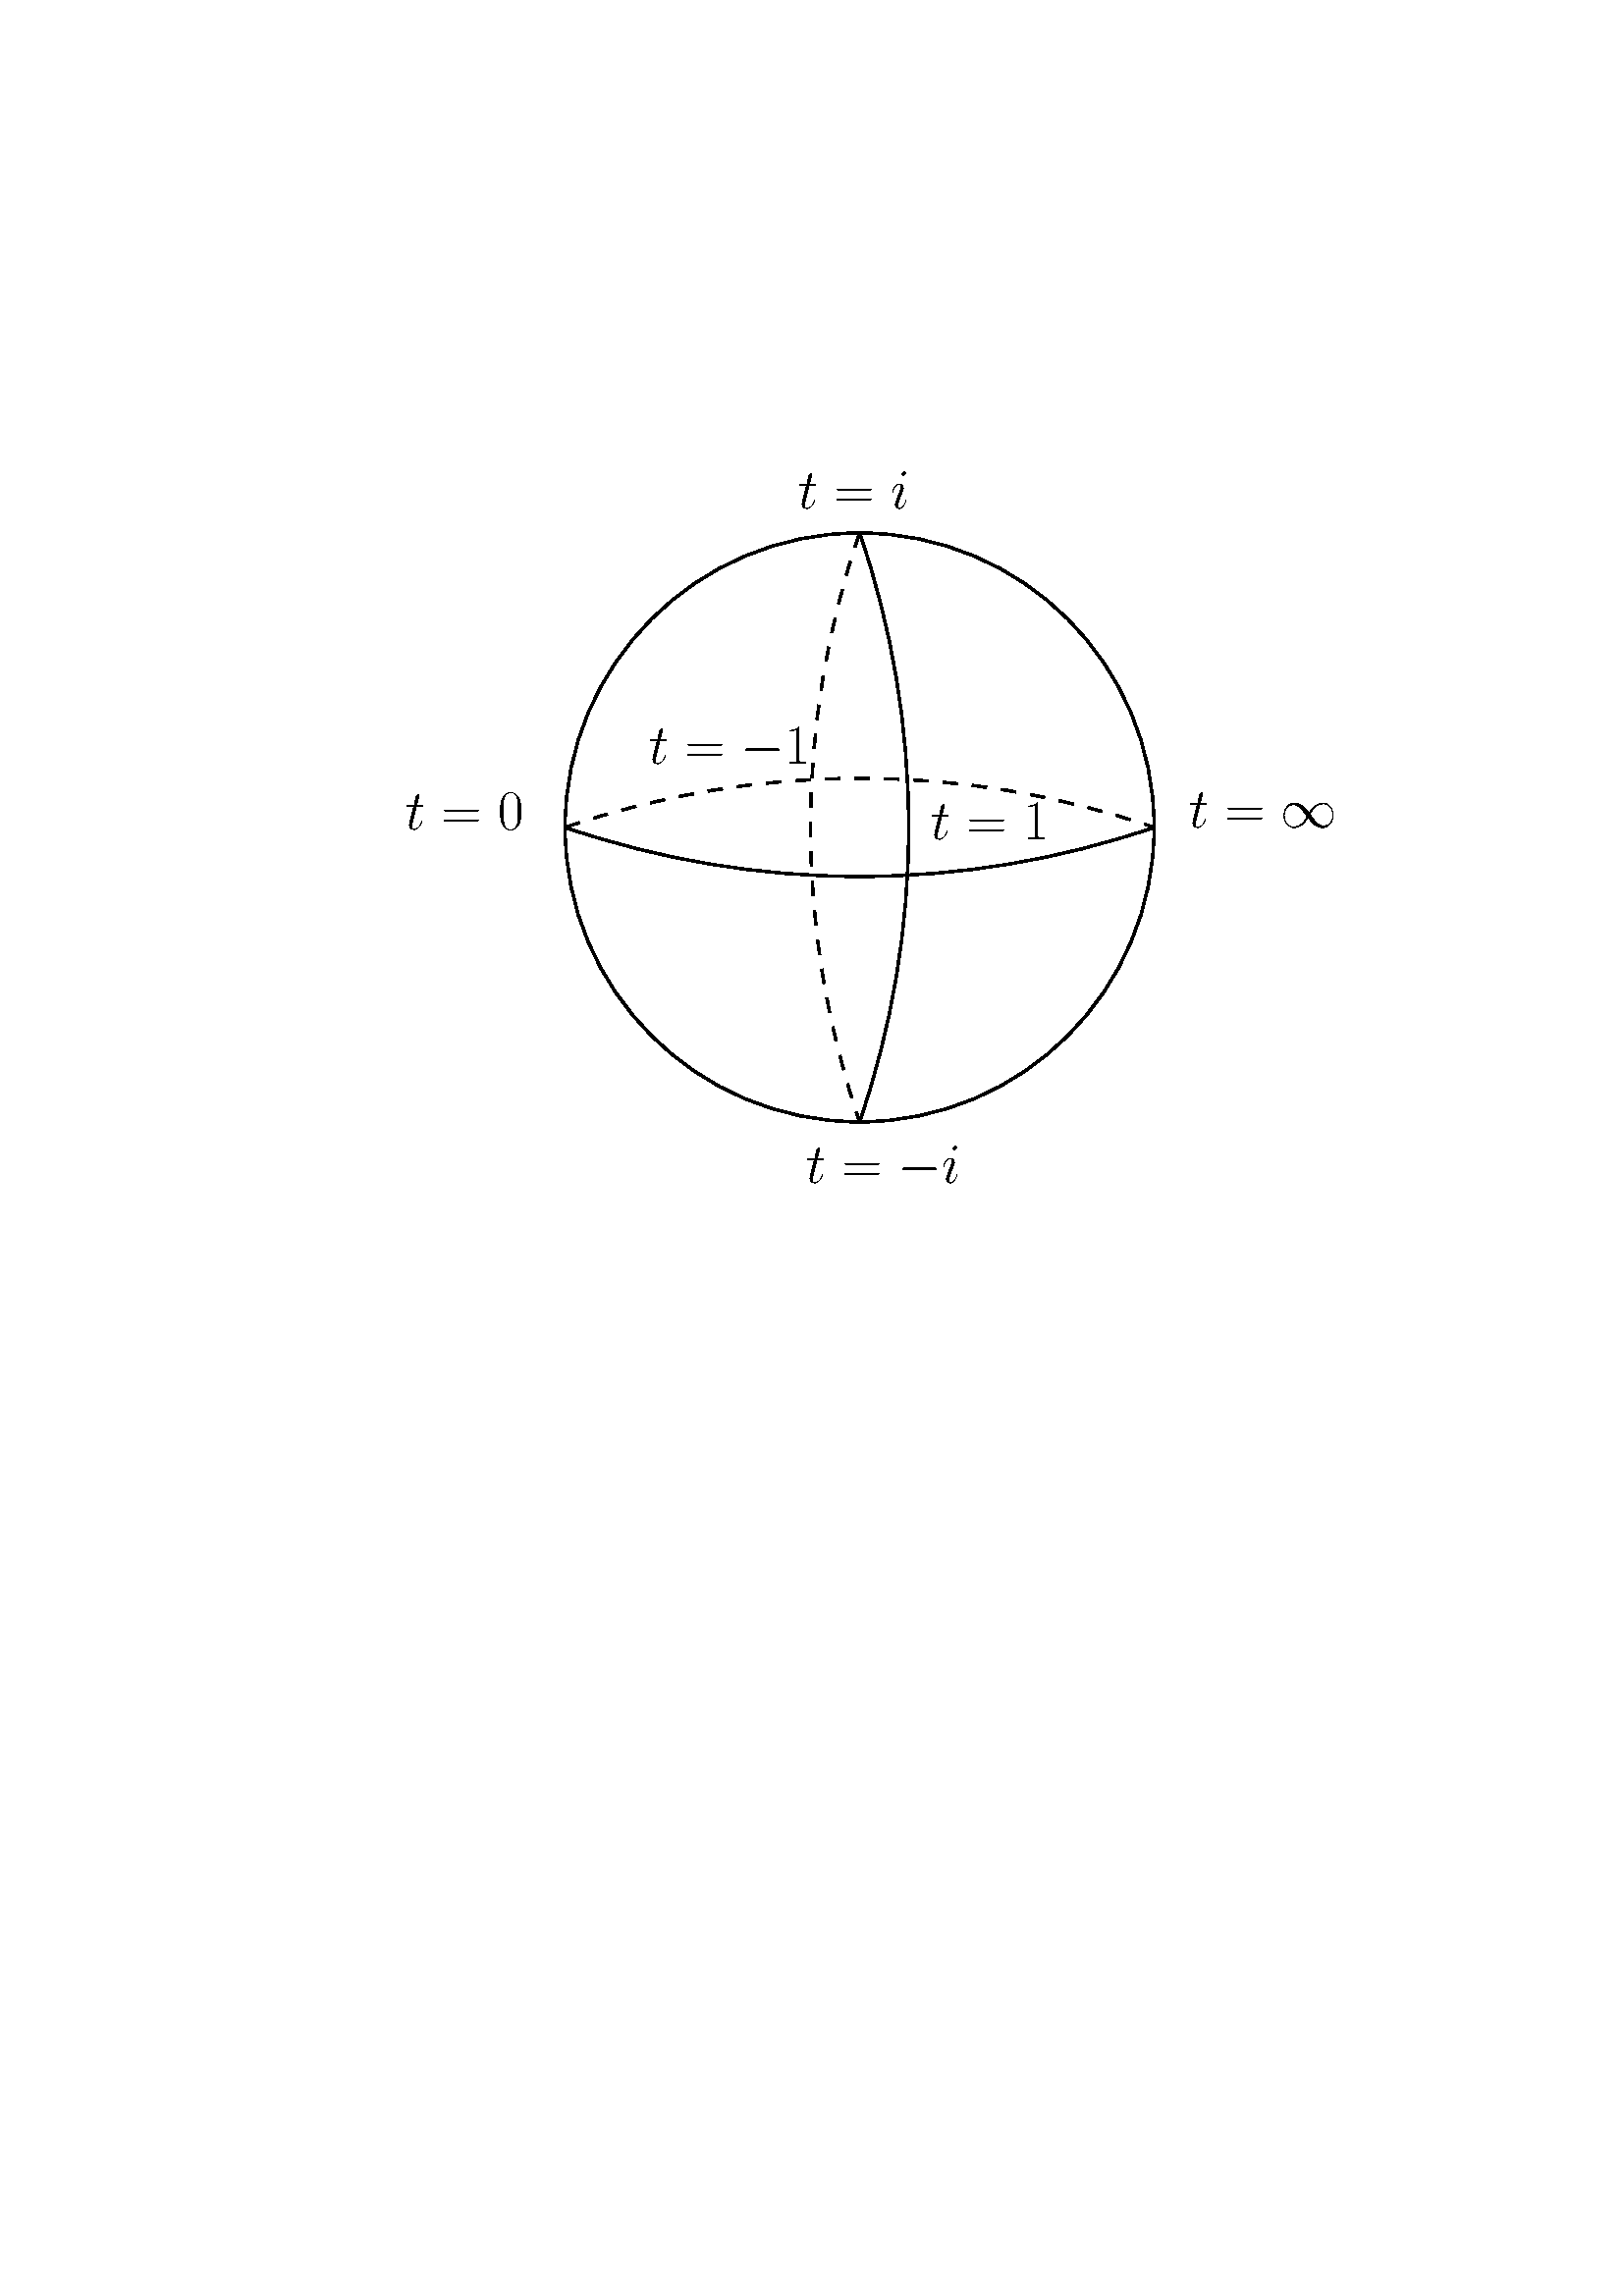
\includegraphics[width=0.75\linewidth]{figures/gla0-1.png}
\caption{ \medskip 以变量 $t$ 为参数的一族拓扑场论。（原文 Fig.~1）}
\label{fig:zunko}
\end{figure}

$Spin'(4)$ 的生成元是 $\Gamma_{\mu\nu}+\Gamma_{\mu+4,\nu+4}$（$\mu,\nu=0,\dots,3$），因此 $Spin'(4)$-不变旋量 $\epsilon$ 满足 $(\Gamma_{\mu\nu}+\Gamma_{\mu+4,\nu+4})\epsilon=0$。取 $\mu,\nu=0,1$，可知 $\Gamma_{0145}\epsilon=\epsilon$；取 $\mu,\nu=2,3$，可知 $\Gamma_{2367}\epsilon=\epsilon$。于是 $\Gamma_0\Gamma_1\dots\Gamma_7\epsilon=\epsilon$；再利用式~\eqref{eq:nohinks} 的手征条件 $\Gamma_0\Gamma_1\dots\Gamma_9\epsilon=-i\epsilon$，可知
% 式 (3.11)
\setcounter{equation}{10}
\begin{equation}\label{eq:banother}
\Gamma_{89}\epsilon=-i\epsilon.
\end{equation}
特别地，由此可知 ${\cal K}=\Gamma_{89}$ 在 $\epsilon_\ell$ 与 $\epsilon_r$ 上以相同的本征值 ${\EUK}=-i{\cal K}=-1$ 作用。还可知 $\Gamma_{8-i9}\epsilon=0$，其中 $\Gamma_{8-i9}=(\Gamma_8-i\Gamma_9)/\sqrt 2$。这些事实有助于验证下文给出的超对称变换律。

现在我们可以看出，为什么这一构造给出以 $\Bbb{CP}^1$ 为参数的一族拓扑场论（\zunko）。我们取 $\epsilon_\ell$ 与 $\epsilon_\rr$ 的任意非零复线性组合 % 式 (3.12)
\setcounter{equation}{11}
\begin{equation}\label{eq:utu}
\epsilon=u\epsilon_\ell+v\epsilon_\rr,
\end{equation}

并把它取作拓扑对称的生成元。对 $\epsilon$ 作整体标度无关紧要，因此拓扑对称的可能选取由 $\Bbb{CP}^1$ 参数化。由于给定 $\epsilon_\ell$ 后 $\epsilon_\rr$ 有自然的选取，这里比一个抽象的 $\Bbb{CP}^1$ 有更多的结构：它带有自然的仿射参数 $t=v/u$。

我们可以用式~\eqref{eq:tokio} 确定 $u$、$v$ 与 $t$ 在 $S$-对偶下的变换。在对偶群 $\Gamma$ 的元素 $\gamma$ 下，有 $\epsilon_\ell\to\exp(i\hat\phi(\gamma))\epsilon_\ell$，$\epsilon_\rr\to\exp(-i\hat\phi(\gamma))\epsilon_\rr$。因此，要保证 $\epsilon=u\epsilon_\ell+v\epsilon_\rr$ 不变，需有 $u\to\exp(-i\hat\phi(\gamma))u$、$v\to\exp(i\hat\phi(\gamma))v$；最终 $t=v/u$ 的变换为

\begin{yizhu}[含糊点拨]
按：式~\eqref{eq:duco} 给出的 $t\mapsto\exp(2i\hat\phi(\gamma))t=\frac{c\tau+d}{|c\tau+d|}t$，与 Frenkel 2009 综述（Séminaire Bourbaki 1010）第 4 节中的 $t\mapsto\frac{\tau}{|\tau|}t$ 相差一个负号：在 $S$-对偶 $\tau\mapsto-1/\tau$ 下，$\frac{c\tau+d}{|c\tau+d|}=\frac{-1/\tau}{1/|\tau|}=-\frac{\tau}{|\tau|}$。两者并不矛盾，因为本文马上就说明 $t$ 与 $-t$ 给出等价的拓扑场论（式~\eqref{eq:ungu}），这个负号被那个平凡等价吸收。记录这一点是因为：不同文献对 twisting parameter 的归一化可能相差一个符号或整体标度，比较公式之前务必先对齐约定。
\end{yizhu} % 式 (3.13)
\setcounter{equation}{12}
\begin{equation}\label{eq:duco}
t\to
\exp(2i\hat\phi(\gamma))t={{c\tau+d}\over\ {|c\tau+d|}}t.
\end{equation}

类似地，我们可以确定 $SU(4)_{{\cal R}}$ 的中心在 $t$ 上的作用。中心的生成元 ${\EUI}$ 按 $\epsilon_\ell\to i\epsilon_\ell$、$\epsilon_\rr\to i^{-1}\epsilon_\rr$ 作用，因此与上面类似的推理给出 % 式 (3.14)
\setcounter{equation}{13}
\begin{equation}\label{eq:ungu}
{\EUI}(t)=-t.
\end{equation}

因此，参数为 $t$ 的拓扑场论与参数为 $-t$ 的拓扑场论彼此等价。这是一种平凡的等价，含义是它来自经典作用量的对称性——而不是来自非平凡的 $S$-对偶。$\Bbb{Z}_2$ 对称性~\eqref{eq:ungu} 是以 $t$ 参数化的一族扭化拓扑场论中唯一的平凡等价。作此断言时，关键的一点是 $\epsilon_\ell$ 与 $\epsilon_\rr$ 具有相同的 ${\cal K}$ 本征值。否则，由 ${\cal K}$ 生成的群 $\Bbb{C}^*$ 中的一个变换将非平凡地作用在 $t$ 上，从而使得整个以 $\Bbb{CP}^1$ 为参数的拓扑场论族都平凡地等价。当然，正因为（几乎）没有平凡等价，来自 $S$-对偶的非平凡等价才有可能生成像几何 Langlands 纲领那样有趣的东西。

\begin{yizhu}[易错点]
按：$t\sim-t$ 是唯一的平凡等价，这句话的分量全在「唯一」二字。理由本段已经给出，但值得用群论重述一遍：如果 $\epsilon_\ell$ 与 $\epsilon_\rr$ 的 ${\cal K}$ 本征值不同，那么由 ${\cal K}$ 生成的连通群 $\Bbb{C}^*$ 会连续地移动 $t$，把 $\Bbb{CP}^1$ 上的每个参数都推入同一个等价类，整族理论随之平凡化，$S$-对偶带来的对偶性也就无从谈起。正因为两者本征值相同（都等于 $-1$，见式~\eqref{eq:banother}），连通的 $\Bbb{C}^*$ 在 $t$ 上作用平凡，只剩下中心元给出的离散 $\Bbb{Z}_2$：$t\mapsto-t$。
\end{yizhu}

我们把由 $\epsilon_\ell$ 与 $\epsilon_\rr$ 生成的超对称记作 $Q_\ell$ 与 $Q_\rr$。由线性组合 $\epsilon=u\epsilon_\ell+v\epsilon_\rr$ 生成的超对称则是 % 式 (3.15)
\setcounter{equation}{14}
\begin{equation}\label{eq:hut}
Q=uQ_\ell+vQ_\rr,
\end{equation}
这就是扭化理论的拓扑对称。写下如下记号也很方便：
% 式 (3.16)
\setcounter{equation}{15}
\begin{equation}\label{eq:nut}
\delta_T=\epsilon_\ell\delta_\ell+\epsilon_\rr\delta_\rr,
\end{equation}

其中对任意场 $\Phi$，
% 式 (3.17)
\setcounter{equation}{16}
\begin{equation}\label{eq:but}
\delta_T\Phi=[Q,\Phi\},~~~\delta_\ell\Phi=
[Q_\ell,\Phi\},~~~\delta_\rr\Phi=[Q_\rr,\Phi\}.
\end{equation}
（$T$ 表示 twisted 或 topological。）由于 $\epsilon_\ell$ 与 $\epsilon_r$ 具有 ${\EUK}=-1$，可知 $Q_\ell$、$Q_\rr$ 与 $Q$ 都具有 ${\EUK}=1$。事实上，下文给出的超对称变换律明确显示，$\delta_T$ 把每个场的 ${\EUK}$ 都提高 $1$。因此在数学语言中，规范不变算子或态构成一个复形，它按 ${\EUK}$ 作 $\Bbb{Z}$-分次，微分是 $Q$。

\begin{yizhu}[易错点]
按：这里的 ${\EUK}$ 记账是全文最容易出错的地方：扭化旋量 $\epsilon_\ell,\epsilon_\rr$ 的 ${\EUK}=-1$，而由它们生成的超荷 $Q_\ell,Q_\rr,Q$ 的 ${\EUK}=+1$；因为 $\delta_T\Phi=[Q,\Phi\}$，$\delta_T$ 把每个场的 ${\EUK}$ 提高 $1$。于是费米场与玻色场的配对不按自旋，而按 ${\EUK}$ 的奇偶：${\EUK}=1$ 的费米场（$\psi,\tilde\psi$）是 $Q$ 的搭档，${\EUK}=-1$ 的（$\chi^\pm,\eta,\tilde\eta$）出现在 $\delta_T$ 的右边。这也解释了为什么 $\sigma$（${\EUK}=2$）在 $\delta_T$ 下不变：要把它映到某个 ${\EUK}=3$ 的场，而理论中没有这样的场。
\end{yizhu}

\par\medskip{\it 费米场与超对称变换}

费米场 $\lambda$ 与超对称生成元 $\epsilon$ 按同样的方式变换，因此利用式~\eqref{eq:lollypop} 与式~\eqref{eq:tollypop}，可以用四维语言识别它们。具有 ${\EUK}=1$ 的场是两个 $({\bf 2},{\bf 2})^1$ 的拷贝，对应两个 1-形式 $\psi$ 与 $\tilde\psi$。按 $({\bf 3},{\bf 1})^{-1}$ 与 $({\bf 1},{\bf 3})^{-1}$ 变换的场，是 ${\EUK}=-1$ 的 2-形式 $\chi$ 的自对偶部分与反自对偶部分 $\chi^\pm$。最后，还有两个 ${\EUK}=-1$ 的零形式 $\eta$ 与 $\tilde\eta$。

为把这些四维场定义得更精确，一个有用的办法是指定十维旋量场 $\lambda$ 按四维费米场的如下展开：\footnote{由于 $\lambda$、$\epsilon_\ell$ 与 $\epsilon_\rr$ 都是正手征的，这一展开只能使用 Clifford 代数的偶元素。为保证这一点，展开中包含若干个因子 $\Gamma_{8+i9}={1\over \sqrt 2}\left(\Gamma_8+ i \Gamma_9\right)$。}
 % 式 (3.18)
\setcounter{equation}{17}
\begin{equation}\label{eq:iko}
\begin{aligned}\lambda=&\left(\eta
+\sum_\mu\Gamma^\mu\psi_\mu \Gamma_{8+i9}
+\sum_{\mu<\nu}\Gamma^{\mu\nu}\chi^+_{\mu\nu}\right)\epsilon_\ell
\\+& \left(\tilde\eta +\sum_{\mu}\Gamma^\mu\tilde\psi_\mu
\Gamma_{8+i9}+\sum_{
\mu<\nu}\Gamma^{\mu\nu}\chi^-_{\mu\nu}\right)\epsilon_\rr.\\\end{aligned}
\end{equation}

这个公式用 $\lambda$ 的十六个分量唯一地确定了十六个场（$\eta$ 与 $\tilde\eta$，$\psi$ 与 $\tilde\psi$ 各四个分量，以及 $\chi$ 的六个分量）。注意，由于 $\hat\Gamma_E\epsilon_\ell=-\epsilon_\ell$，$\Gamma_{\mu\nu}\epsilon_\ell$ 是自对偶的，因此 $\Gamma^{\mu\nu}\chi_{\mu\nu}\epsilon_\ell=\Gamma^{\mu\nu}\chi^+_{\mu\nu}\epsilon_\ell$。同样，$\Gamma^{\mu\nu}\chi_{\mu\nu}\epsilon_\rr=\Gamma^{\mu\nu}\chi^-_{\mu\nu}\epsilon_\rr$。所以在式~\eqref{eq:iko} 中可以把 $\chi^\pm$ 等价地换成 $\chi$。

方便的做法是把 $\epsilon_\ell$ 归一化（允许差一个符号），使得
% 式 (3.19)
\setcounter{equation}{18}
\begin{equation}\label{eq:zomop}
\bar\epsilon_\ell \Gamma_{8+i9}\epsilon_\ell = 1.
\end{equation}
于是由 $\epsilon_r=N\epsilon_\ell$ 同样可得
% 式 (3.20)
\setcounter{equation}{19}
\begin{equation}\label{eq:omop}
\bar\epsilon_r\Gamma_{8+i9}\epsilon_r=1.
\end{equation}
由四维手征性的考虑可得
% 式 (3.21)
\setcounter{equation}{20}
\begin{equation}\label{eq:tomop}
\bar\epsilon_\ell\Gamma_{8+i9}\epsilon_r
=\bar\epsilon_r\Gamma_{8+i9}\epsilon_\ell=0.
\end{equation}

下一步是描述各场在拓扑对称（即由 $\epsilon_\ell$ 与 $\epsilon_\rr$ 生成的超对称）下如何变换。例如，要变换玻色子，我们从 $\delta_S A_I=i\bar\epsilon\Gamma_I\lambda$ 出发。令 $\epsilon=u\epsilon_\ell+v\epsilon_\rr$，就得到四维规范场的变换 % 式 (3.22)
\setcounter{equation}{21}
\begin{equation}\label{eq:kono}
\delta_T A_\mu = iu\bar \epsilon_\ell
\Gamma_\mu \lambda +iv\bar\epsilon_\rr\Gamma_\mu\lambda.
\end{equation}
经过一番 $\Gamma$-矩阵运算，可以得到四维规范场在拓扑超对称下的变换： % 式 (3.23)
\setcounter{equation}{22}
\begin{equation}\label{eq:bono}
\delta_T A_\mu=iu
\psi_\mu+iv\tilde\psi_\mu.
\end{equation}
类似地，对其他玻色场我们得到 % 式 (3.24)
\setcounter{equation}{23}
\begin{equation}\label{eq:lono}
\delta_T\phi_\mu=iv\psi_\mu -
iu\tilde\psi_\mu.
\end{equation}
 % 式 (3.25)
\setcounter{equation}{24}
\begin{equation}\label{eq:otono}
\begin{aligned}\delta_T\sigma & = 0 \\
                       \delta_T\bar\sigma & = iu\eta+iv\tilde\eta.\\\end{aligned}
\end{equation}

$\delta_T\sigma$ 之所以为零，其实只源于 $\sigma$ 具有 ${\EUK}=2$，而并不存在 ${\EUK}=3$ 的合适场。

同样地，我们可以从基本的变换律出发，求出四维费米场的变换：
% 式 (3.26)
\setcounter{equation}{25}
\begin{equation}\label{eq:invo}
\delta_T\lambda=\half\sum_{I,J=0}^9F_{IJ}\Gamma^{IJ}\epsilon,
\end{equation}

其中 $\epsilon=u\epsilon_\ell+v\epsilon_\rr$。具有 ${\EUK}=-1$ 的费米场的变换为
% 式 (3.27)
\setcounter{equation}{26}
\begin{equation}\label{eq:helpme}
\begin{aligned}\delta_T\chi^+ & = u(F-\phi\wedge\phi)^+
+v(D\phi)^+\\ \delta_T\chi^-& = v(F-\phi\wedge\phi)^- -
u(D\phi)^-\\ \delta_T\eta& = vD^*\phi+u[\bar\sigma,\sigma] \\
\delta_T\tilde\eta& = -uD^* \phi+v[\bar\sigma,\sigma].\\\end{aligned}
\end{equation}
具有 ${\EUK}=1$ 的那些场的变换为 % 式 (3.28)
\setcounter{equation}{27}
\begin{equation}\label{eq:mimo}
\begin{aligned}\delta_T\psi& = u\,
D\sigma +v[\phi,\sigma]\\ \delta_T\tilde\psi & = v\, D\sigma - u
[\phi,\sigma].\\\end{aligned}
\end{equation}
在这些公式中，$D=d+[A,\,\cdot \,]$ 是相对于联络 $A$ 的协变导数；在伴随丛取值的 2-形式 $\phi\wedge\phi$ 中隐含着一个李括号；而 $D^*\phi=\star D \star \phi=D_\mu\phi^\mu$，其中 $\star$ 是 Hodge 星算子。
